An axis aligned rectangle classifier is a classifier than assigns the value 1 to a point if and only if it is inside a certain rectangle. Formally, given real numbers $a_1\le b_1, a_2 \le b_2$, define the classifier $f_{(a_1,b_1,a_2,b_2)}$ on an input $\x$ with coordinates $(x_1,x_2)$ by
    \[ 
    f_{(a_1,b_1,a_2,b_2)}(x_1, x_2) =
    \begin{cases} 
      1 & \text{if } a_1\le x_1\le b_1 \text{ and }  a_2\le x_2\le b_2\\
      -1 & \text{otherwise}.
   \end{cases}
\]
The function class of all axis-aligned rectangles in the plane is defined as
\begin{align*}
    \mathcal{F}_{\text{rec}}^2 = \{ f_{(a_1,b_1,a_2,b_2)}(x_1, x_2): a_1 \le b_1, a_2 \le b_2\}.
\end{align*}
We will assume that the true labels $y$ of the data points $(\x,y)$ are given by some axis-aligned rectangle (this is the realizability assumption discussed in class). The goal of this question is to come up with an algorithm which gets small classification error with respect to any distribution $D$ over $(\x,y)$ with good probability.

The loss function we use throughout the question is the 0-1 loss. It will be convenient to denote a rectangle marked by corners $(a_1,b_1,a_2, b_2)$ as $B(a_1,b_1,a_2, b_2)$. Let $B^*=B(a_1^*, b_1^*, a_2^*, b_2^*)$ be the rectangle corresponding to the function $f_{(a_1^*, b_1^*, a_2^*, b_2^*)}$ which labels the datapoints (meaning that for all $(\x,y)$ drawn from distribution $D$, $f_{(a_1^*, b_1^*, a_2^*, b_2^*)}(\x)=y$). Let $S=\{(\x_i,y_i), i \in [n]\}$ be a training set of $n$ samples drawn i.i.d. from $D$. 
Please see Fig.~\ref{fig:rect} for an example.\\

\begin{figure}[h]
    \centering
    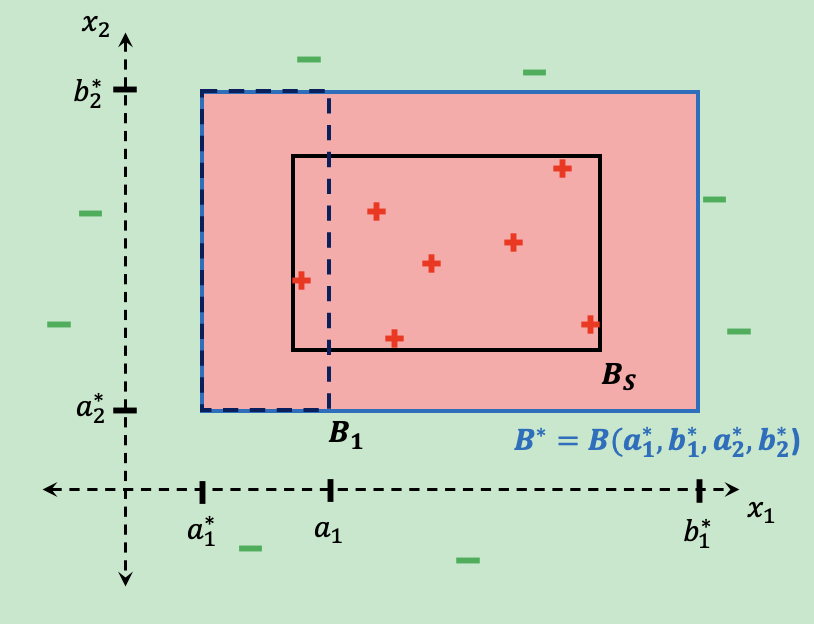
\includegraphics[width=0.5\textwidth]{rect.png}
    \caption{Learning axis-aligned rectangles in two dimensions, here $+$ (red) denotes datapoints in training set $S$ with label 1 and $-$ (green) denotes datapoints with label -1. The true labels are given by rectangle $B^*$ (solid blue line), with everything outside $B^*$ being labelled negative and inside being labelled positive. $B_S$ (solid black line) is the rectangle learned by the algorithm in \textbf{2.2}. $B_1$ (dashed black line) is defined in \textbf{2.3}.}
    \label{fig:rect}
\end{figure}


\textbf{2.1} (\blue{4pts}) We will follow the general supervised learning framework from class. For a function $f_{(a_1,b_1,a_2,b_2)}$, define the empirical risk with respect to 0-1 loss as $\widehat{\mathcal{R}}(f_{(a_1,b_1,a_2,b_2)})=\sum_{i=1}^n\mathbb{I}\{f_{(a_1,b_1,a_2,b_2)}(\x_i)\neq y_i\}$. Given the 0-1 loss, and the function class of axis-aligned rectangles, we want to find an empirical risk minimizer. Consider the algorithm which returns the smallest rectangle enclosing all positive examples in the training set. Prove that this algorithm is an empirical risk minimizer, meaning that it minimize $\widehat{\mathcal{R}}(f)$ over all $f$ in $\mathcal{F}_{\text{rec}}^2$. (\emph{Hint: use the realizability assumption.})\\

\noindent{\fontsize{11}{12}\selectfont\textbf{Solution 2.1}}

Since the algorithm returns the \textbf{smallest} rectangle enclosing all positive examples, we suppose it as $B_S$.

By the definition of $B^*$ in the description of Figure 1, we know that everything outside $B^*$ being labeled negative and inside being labeled positive.

Therefore, we have:
\[
B_S \subseteq B^*
\]

Define $S_+$ as the set of all positive examples:
\[
S_+ = \{\mathbf{x}_i \in S, y_i = 1\}
\]

Thus,
\[
\forall \mathbf{x}_i \in S_+ , \mathbf{x}_i \in B_S ,
\]

which means for all $\mathbf{x}_i$, 
\[
f_{B_S}(\mathbf{x}_i) = 1
\]

Define:
\[
S_- = \{\mathbf{x}_j \in S, y_j = -1\}
\]

Since
\[
\mathbf{x}_j \notin B^*
\]

Therefore,
\[
x_j \notin B_S
\]
\[
f_{B_S}(\mathbf{x}_j) = -1
\]

So We have
\[
\hat{R}(f_{B_S}(\mathbf{x})) = \frac{1}{n}\sum_{i=1}^n \mathbb{I}\{f_{B_S}(\mathbf{x}) \neq y\} = 0,
\]

which means the algorithm is an empirical risk minimizer.
\bigskip

\textbf{2.2} (\blue{4pts}) Our next task is to show that the algorithm from the previous part not only does well on the training data, but also gets small classification error with respect to the distribution $D$.  Let $B_S$ be the rectangle returned by the algorithm in \textbf{2.1} on training set $S$, and let $f_S^{ERM}$ be the corresponding hypothesis. First, we will convince ourselves that generalization is inherently a probabilistic statement. Let a \emph{bad} training set $S'$ be a training set such that $R(f_{S'}^{ERM})\ge 0.5$. Pick some simple distribution $D$ and ground-truth rectangle $B^*$, and give a short explanation for why there is a \emph{non-zero} probability of seeing a bad training set.\\

\noindent{\fontsize{11}{12}\selectfont\textbf{Solution 2.2}}

Let us pick a discrete uniform distribution D as small as there are only 3 positive examples $(\mathbf{x}_1, \mathbf{x}_2, \mathbf{x}_3)$ within $B^*$ and 1 negative example $(\mathbf{x}_4)$ outside $B^*$. $\mathbf{x}_i$ are with coordinates $(x_1, x_2)$.

\[
D = \{\mathbf{x}_1, \mathbf{x}_2, \mathbf{x}_3, \mathbf{x}_4\}
\]

Suppose that the size of $S'$ is 1, which is a bad training set. 

Therefore, each point has a probability of

\[
P(\mathbf{x}_i) = 0.25
\]

If $S'$ only contains $\{\mathbf{x}_1\}$, then the algorithm in \textbf{2.1} returns a tiny rectangle $B_{S'}$ that only covers $\mathbf{x}_1$. And $B_{S'}$ will misclassify $\mathbf{x}_2$ and $\mathbf{x}_3$ as negative.

Then
\[
R(f_{S'}^{ERM}) = P(\mathbf{x}_2) + P(\mathbf{x}_3) = 0.25 + 0.25 = 0.5.
\]

Since the examples are picked from distribution (i.i.d.) and the size of set $S'$ is not big enough, there is always a non-zero probability of seeing a bad training set, where all positive samples are concentrated in a local subregion of $B^*$. This will cause the minimum rectangle generated by the algorithm in \textbf{2.1} to be too narrow, resulting in errors for other unseen positive samples.
\bigskip

\textbf{2.3} (\blue{8pts})  Though there is non-zero probability seeing bad training set, we will now show that \emph{with high probability} over the training dataset $S$, $f_S^{ERM}$ \emph{does} get small error. Show that if $n\ge \frac{4 \log (4/\delta)}{\epsilon}$ then with probability at least $1-\delta$, $R(f_S^{ERM})\le \epsilon$.
    
    To prove this follow the following steps. Let $a_1 \ge a_1^*$ be such that the probability mass (with respect to $D$) of the rectangle $B_1=B(a_1^*, a_1, a_2^*, b_2^*)$ is exactly $\epsilon/4$. Similarly, let $b_1\leq b_1^*, a_2\geq a_2^*,b_2\leq b_2^*$ be numbers such that the probability mass (with respect to $D$) of the rectangles $B_2=B(b_1,b_1^*, a_2^*, b_2^*), B_3=B(a_1^*, b_1^*, a_2^*, a_2), B_4=B(a_1^*, b_1^*, b_2, b_2^*)$ are all exactly $\epsilon/4$.
    \begin{itemize}
        \item Show that $B_S \subseteq B^*$.
        \item Show that if $S$ contains (positive) examples in all of the rectangles $B_1, B_2, B_3, B_4$ then $R(f_S^{ERM})\le \epsilon$. (Hint: think about the geometric relationship between $B_i$ and $B_S$, $i\in\{1,2,3,4\}$)
        \item For each $i \in \{1,\dots, 4\}$ upper bound the probability that $S$ does not contain an example from $B_i$.
        \item Use the union bound to conclude the argument.
    \end{itemize}

\noindent{\fontsize{11}{12}\selectfont\textbf{Solution 2.3}}

\bigskip

\textbf{(Bonus) 2.4} (\blue{8pts}) Repeat the previous question for the function class of axis-aligned rectangles in $\R^d$. Specifically, the current function class is $\mathcal{F}_{\text{d-rec}}=\{f_{(a_1,b_1,a_2,b_2,\dots,a_d,b_d)}(x_1,x_2,\dots,x_d):a_i\leq b_i, i\in\{1,2,\dots,d\}\}$ and a datapoint $\x\in\R^d$ is predicted to be $1$ by $f_{(a_1,b_1,a_2,b_2,\dots,a_d,b_d)}(x_1,x_2,\dots,x_d)$ if $a_i\leq x_i\leq b_i$ for all $i\in\{1,2,\dots,d\}$ and $-1$ otherwise. We will still assume realizability. To show this, try to generalize all the steps in the above question to higher dimensions, and find the number of training samples $n$ required to guarantee that $R(f_S^{ERM})\le \epsilon$ with probability at least $1-\delta$. \\

\noindent{\fontsize{11}{12}\selectfont\textbf{Solution 2.4}}

\bigskip